\def\year{2020}\relax
%File: formatting-instruction.tex
\documentclass[letterpaper]{article} %DO NOT CHANGE THIS
\usepackage{aaai20}  %Required
\usepackage{times}  %Required
\usepackage{helvet}  %Required
\usepackage{courier}  %Required
\usepackage{url}  %Required
\usepackage{graphicx}  %Required
\frenchspacing  %Required
\setlength{\pdfpagewidth}{8.5in}  %Required
\setlength{\pdfpageheight}{11in}  %Required
\pdfinfo{
/Title (Privacy Preserving Planning in Stochastic Environments)
/Author (Guy Shani, Roni Stern, Tommy Hefner)}
\usepackage{booktabs}
\usepackage{xspace}
\usepackage{amsmath,amssymb}
\usepackage{eurosym}
% Use the postscript times font!
\usepackage{times}
\usepackage{mathtools}
\usepackage{soul}
\usepackage{url}
%\usepackage[hidelinks]{hyperref}
\usepackage[utf8]{inputenc}
\usepackage{graphicx}
\usepackage{amsmath}
\usepackage{amsfonts}
\usepackage{amssymb}
\usepackage{amsthm}
\usepackage{booktabs}
\usepackage[ruled,linesnumbered,noend]{algorithm2e}
\usepackage{amsthm}   
\usepackage{pgfplots,graphicx}
%\usepackage{subfigure}
% Use the postscript times font!
\usepackage{times}
\usepackage{soul}
\usepackage{url}
\usepackage[utf8]{inputenc}
\usepackage{graphicx}
\usepackage{amsmath}
\usepackage{booktabs}
\usepackage{algorithmic}
\usepackage{thmtools}
\usepackage{subcaption}

%\setlength{\intextsep}{5pt} % Vertical space above & below [h] floats % todo - we cannot use intextsep according to AAAI formatting standard
%\setlength{\textfloatsep}{5pt} % Vertical space below (above) [t] ([b]) floats
%\setlength{\abovecaptionskip}{10pt}
%\setlength{\belowcaptionskip}{0pt}


\newcommand{\mafs}{\textsc {mafs}\xspace}
\newcommand{\smafs}{\textsc {smafs}\xspace}
\newcommand{\fmafs}{\textsc {mafbs}\xspace}
\newcommand{\mafbs}{\textsc {mafbs}\xspace}
\newcommand{\smafbs}{\textsc {smafbs}\xspace}
\newcommand{\mastrips}{\textsc {ma-strips}\xspace}
\newcommand{\cppp}{\textsc {cppp}\xspace}
\newcommand{\scppp}{\textsc {scppp}\xspace}
\newcommand{\rtdp}{\textsc {rtdp}\xspace}
\newcommand{\drtdp}{\textsc {drtdp}\xspace}
\newcommand{\psrtdp}{\textsc{ps}-\textsc{rtdp}\xspace}
\newcommand{\mdps}{\textsc {mdp}s\xspace}
\newcommand{\mdp}{\textsc {mdp}\xspace}


\urlstyle{same}
\usepackage{array}
\newcolumntype{L}{>{\centering\arraybackslash}m{3cm}}
\newcommand{\tommy}[1]{\textbf{[\color{red}TOMMY:#1]}}
\newcommand{\roni}[1]{\textbf{[\color{blue}RONI:#1]}}
\newcommand{\guy}[1]{\textbf{[\color{orange}GUY:#1]}}

\declaretheorem{theorem} 
\declaretheoremstyle[%
  spaceabove=0pt,%
  spacebelow=0pt,%
  headfont=\normalfont\itshape,%
  postheadspace=1em,%
  qed=\qedsymbol%
]{mystyle} 
\declaretheorem[name={Proof},style=mystyle,unnumbered,
]{prf}
\usepackage{adjustbox}

\theoremstyle{remark}
\newtheorem{definition1}{Definition}
\newtheorem{example}{Example}
\newtheorem{lemma}{Lemma}
\newtheorem{proposition}{Proposition}
\newcolumntype{R}[2]{%
    >{\adjustbox{angle=#1,lap=\width-(#2)}\bgroup}%
    l%
    <{\egroup}%
}

\newcommand*\rot{\multicolumn{1}{R{45}{1em}}}
\newcommand{\citet}[1]{\citeauthor{#1}~\shortcite{#1}}
\newcommand{\citep}[1]{\cite{#1}}

\newcommand{\commentout}[1]{}
\newcommand{\move}[0]{\mbox{{\em move}}}
% the following package is optional:
%\usepackage{latexsym} 


\setcounter{secnumdepth}{2}

\title{Privacy Preserving Planning in Stochastic Environments}
 
\author{Guy Shani, Roni Stern, and Tommy Hefner\\
Ben Gurion University of the Negev, SISE Dept., Be’er Sheva, Israel}

\begin{document}

\maketitle

\begin{abstract}

Collaborative privacy preserving planning (\cppp) has gained much attention in the past decade. To date, \cppp\ has focused on domains with deterministic action effects. In this paper, we extend \cppp\ to domains with stochastic action effects. We show how such environments can be modeled as an \mdp. We then focus on the popular Real-Time Dynamic Programming (RTDP) algorithm for computing value functions for \mdps, extending it to the stochastic \cppp\ setting. We provide two versions of RTDP: a complete version identical to executing centralized RTDP, and an approximate version that sends significantly fewer messages and computes competitive policies in practice. We experiment on domains adapted from the deterministic \cppp\ literature.
\end{abstract}



\section{Introduction}

Designing autonomous agents that act collaboratively is an important goal. A fundamental requirement of such collaboration is to plan for multiple agents acting to achieve a common set of goals.  \emph{Collaborative privacy-preserving planning (\cppp\ )} is a multi-agent planning task in which agents need to achieve a common set of goals without revealing certain private information~\citep{brafman2008one}. In particular, in \cppp\  an individual agent may have a set of private facts and actions that it does not share with the other agents. \cppp\  has important motivating examples, such as planning for organizations that outsource some of their tasks.

In this paper we extend the \cppp\ framework to stochastic domains, where actions may have different effects with varying probabilities. In the planning community, stochastic domains are typically modeled using Markov decision processes (\mdps) \cite[e.g.]{kolobov2012planning}. We suggest an \mdp formalization for privacy preserving stochastic problems. 

A popular approach for solving goal based \mdps is the Real-Time Dynamic Programming (\rtdp) algorithm~\cite{barto1995learning}, computing a value function, estimating the expected cost to the goal from each state. \rtdp executes trajectories in the state space, updating the value function along the trajectory, and is guaranteed, under some restrictions, to converge to the optimal value function. We adapt \rtdp to our stochastic \cppp\ setting, showing how agents execute jointly state space trajectories, resulting in the distributed \rtdp algorithm (\drtdp).

The complete version of \drtdp follows the same trajectories that will be computed on a centralized \mdp. To do so, \drtdp requires a constant synchronization between the agents, which results in many messages. We thus suggest an approximate \drtdp version that requires synchronization only following public actions, which we call the Public Sync \rtdp~ (\psrtdp). This approximate \drtdp is not guaranteed to converge, and in particular, its trajectories may get into private cycles, requiring restarting the trajectory. 

We compare the two versions over a set of domains adapted from the deterministic \cppp\ literature \cite{vstolba2015competition}, showing that both versions converge to similar expected costs, while \psrtdp requires as much as an order of magnitude fewer messages.



\section{Background} 

We briefly review background on \cppp, \mdps, and \rtdp.

\subsubsection{Collaborative Privacy Preserving Planning}

An \mastrips\ problem~\citep{BrafmanD13} is represented by a tuple $\langle P, \{A_i\}_{i=1}^k, I ,G \rangle$ where:
$k$ is the number of agents, $P$ is a finite set of primitive propositions (facts), $A_i$ is the set of actions agent $i$ can perform,  $I$ is the start state, and $G$ is the goal condition.	

\commentout{
Each action $a=\langle pre(a), \mathit{eff}(a) \rangle$ is defined by its preconditions ($pre(a)$), and effects ($\mathit{eff}(a)$). Preconditions and effects are conjunctions of primitive propositions and literals, respectively. A state is a truth assignment over $P$.  $G$ is a conjunction of facts. $a(s)$ denotes the result of applying action $a$ to state $s$. A {\em plan} $\pi=(a_1,\ldots,a_k)$ is a solution to a planning task iff $G\subseteq a_k(\ldots(a_1(I)\ldots)$.
%, i.e., a sequence of actions that transforms the initial state ($I$) to a state satisfying the goal condition ($G$). 
}
Privacy-preserving \mastrips\ extends \mastrips\ by defining sets of variables and actions as private, known only to a single agent. $private_i(P)$ and $private_i(A_i)$ denote the variables and actions, respectively, that are private to agent $i$. $public(P)$ is the set of public facts in $P$. $public_i(A_i)$, the complement of $private_i(A_i)$ w.r.t.~$A_i$, is the set of public actions of agent $i$. Some preconditions and effects of public actions may be private, and the action obtained by removing these private elements is called its {\em public projection\/}, and it is known to other agents. All agents are aware of the execution of a public action, and view the public effects of the action. Goals can be public, or private to one agent.

\commentout{
An agent is aware only of its {\em local view} of the problem --- its private actions and facts, its public actions, the public facts, and the public projection of the actions of all other agents. For public actions of other agents, the local view contains only the public preconditions and effects.


	\begin{figure}[t]
		\centering
		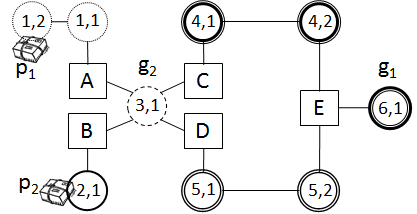
\includegraphics[width=0.3\textwidth]{Logistics}
		\caption{A logistics example. Shared logistics centers are denoted by squares. Cities are denoted by circles, labeled by a pair $i,j$ where $i$ is the agent covering this city and $j$ is the city index. 
		}
		\label{fig:logistics}
	\end{figure}
	

In the logistics example in Figure~\ref{fig:logistics}, the set of facts $P$ represents the location of two packages and six trucks. Each truck has three actions: move, load, and unload, corresponding to moving  between locations, loading a package and unloading it. 
Trucks can only drive along the edges in Figure~\ref{fig:logistics}. Agents have restricted range, such that location $i,j$ can only be reached using truck $i$. The rectangles are logistic centers visited by multiple trucks that load or unload packages. 

Trucks do not want to share their locations and coverage (the locations that a truck can reach). Thus, all the facts representing the location of trucks are private, while the facts representing whether a package is at a logistic center are public. Only the load/unload actions at the logistic centers are public, whereas the move actions are private for each agent, as well as loading and unloading at private locations.  
}

\mafs\ \citep{nissim2014distributed} is a popular algorithm for \cppp\ --- a distributed algorithm in which every agent runs a best-first search to reach the goal. Agents maintain an open list of states, and in every iteration choose a state from the open list to expand, generating all its children and adding them to the open list (avoiding duplicates). Whenever an agent expands a state that was generated by applying a public action, it also broadcasts this state to all other agents. An agent that receives a state adds it to the open list. 
%For example, in Figure~\ref{fig:logistics}, when agent 1 unloads $p_1$ at $A$, it broadcasts this state to all other agents. Agent 3 can now use this state to load $p_1$ and transport it to logistic centers $B,C$, and $D$.

To preserve privacy, the private part of a state is obfuscated when broadcasting it, e.g., by replacing the private facts with some index, such that only the broadcasting agent knows how to map this state index to the corresponding private facts. Once the goal is reached, the agent achieving the goal informs all others, and the search process stops.
%\mafs\ can be extended in several ways. The MADLA planner, e.g., \citep{MADLA} augments \mafs\ with two different open lists, one ordered by a local heuristic, while the other ordered by a global heuristic. 


\subsubsection{Markov Decision Processes}

In many domains there can be several alternative action effects. First, actions may fail, e.g., in the Logistics domain, loading a package may fail, and the package would remain where it was. Second, actions may have unwanted effects. For example, the driver may enter a wrong destination into the navigation app, and drive to the wrong location. In many cases one can have a stochastic model specifying the probability for each effect to occur.

Such planning domains can be modeled by Markov Decision Processes (\mdps) \cite{kolobov2012planning}. In automated planning, an \mdp is a tuple $\langle P,A,I,G,C \rangle$ where $P$ is a finite set of propositions, $A$ is a finite set of actions, $I$ is the start state, $G$ is the goal condition, and $C$ is a cost function. The set of states of the \mdp $S$ is the set of all possible assignments to the propositions in $P$.
An action $a\in A$ is defined by preconditions $pre(a)$ as above. However, the action effects $\mathit{eff}(a)$ is a set of stochastic effects $\langle \phi_i, p_i \rangle$, where $\phi_i$ is a conjunction of positive and negative literals, and $p_i$ is the probability that this specific effect would occur. As some effect must always occur, $\sum_i p_i = 1$. For a pair of states $s,s'$, we denote by $tr(s,a,s')$ the probability that the agent would arrive at state $s'$ by executing $a$ at state $s$. If $s\models G$, then $tr(s,a,s)=1, \forall a \in A$. That is, goal states are absorbing.
The cost function assigns a cost to executing an action $a$ at a state $s$. The cost for any action at a goal state $s \models G$ is $0$, while executing an action at any other state incurs a positive cost. Hence, the agent strives to arrive at a goal state.

A solution for an \mdp is a policy, a mapping $\pi:S \rightarrow A$, assigning an action to every state. A policy that minimizes the expected cost  for reaching the goal is an optimal solution to an \mdp. 
Many \mdp algorithms compute a policy by first computing a value function $V:S \rightarrow A$ assigning a value to each state, estimating the expected cost for achieving the goal. 
The value iteration algorithm computes a value function by iteratively applying the Bellman update:
\begin{eqnarray}
Q(s,a) &=& C(s,a)+ \sum_{s'} tr(s,a,s') V(s')\\
V(s) &=& min_a Q(s,a)
\end{eqnarray}
over every state until convergence. The resulting policy is:
$\pi^V(s) = argmin_a C(s,a)$.

The RTDP algorithm (Algorithm~\ref{alg:RTDP}) \cite[e.g.]{kolobov2012planning} operates by launching simulated trajectories in state space, starting from the initial state. During a trajectory, at each state $s$, the algorithm selects a heuristically best action $a$, and then selects the next state from the $tr(s,a,\cdot)$ distribution. When RTDP reaches a goal state, the trajectory is terminated, and a new one is launched. Bellman updates are used to update the value function along the trajectory. If the value function is initialized optimistically (e.g. to 0), RTDP converges to the optimal value function.

\begin{algorithm}[t!]
\footnotesize
\caption{RTDP}
    \label{alg:RTDP}
\SetKwBlock{RTDP}{RTDP()}{end}
\RTDP{
    $\forall s \in S, a \in A, Q(s,a) \leftarrow 0, V(s) \leftarrow 0$\\
    \While{$V$ has not converged}{
        $s \leftarrow s_0$\\
        \While{$s \not\models G$}{
            $a^* \leftarrow argmin_a Q(s,a)$\\
            $Q(s,a) = C(s,a) + \sum_{s'} tr(s,a,s') V(s')$\\
            $V(s)\leftarrow min_{a'}Q(s,a')$\\
            sample $s'$ from $tr(s,a^*,\cdot)$\\
            $s \leftarrow s'$
        }
    } 
}
\end{algorithm}
%\vspace{-5pt}





\section{Privacy Preserving MDPs}

We extend the definition of \cppp\ to stochastic domains, modeled as an \mdp, with each agent viewing only a part of the complete \mdp.
More formally, a stochastic collaborative privacy preserving planning problem (\scppp) is a tuple: $\langle P, \{A_i\}_{i=1}^k, tr, I ,G, C \rangle$ where
$k$ is the number of agents, $P$ is a finite set of primitive propositions (facts), $A_i$ is the set of actions agent $i$ can perform,  $I$ is the start state, $G$ is the goal condition, and $C$ is a cost function.
As in a \cppp\  problem, $private_i(P)$ and $private_i(A_i)$ denote private variables and action of agent $i$. $public(P)$ is the set of public facts in $P$, and $public_i(A_i)$ is the set of public actions of agent $i$.
As in an \mdp, actions have stochastic effects, i.e. $\mathit{eff}(a)=\{\langle \phi_i, p_i \rangle\}$ where $p_i$ is the probability that effect $\phi_i$ would occur. As in an \mdp, $C$ assigns a cost for executing an action at a state. $tr$ is a transition function, specifying the probability of moving from states $s$ to $s'$ using action $a$.

While in classical \cppp\ problems a solution is a sequence of public and private actions, in an \scppp\ problem the solution is a policy, determining at each step which agent should execute an action, and which action must be executed. Hence, the policy of an agent $i$ is a mapping  $\pi_i: S_i \rightarrow A_i \cup \{\mathit{noop}\}$, where $S_i$ is the set of local states --- assignments to the private propositions of $i$ and the public propositions. Such a policy either chooses an action to execute at a given state, or lets another agent perform an action. 

In this paper we focus on policies that do not allow parallel execution, that is, for each state $s$ of the system, there is exactly one agent where $\pi_i(s_i) \neq \mathit{noop}$, where $s_i$ is the local view of agent $i$ of the global state $s$. 
We leave extensions that allow for parallel executions where more than one agent executes an action at each step to future research.



\begin{algorithm}[t!]
\footnotesize
\caption{DRTDP for agent $i$}
\label{alg:DRTDP}
\SetKwBlock{DRTDP}{DRTDP($i$)}{end}
\SetKwBlock{process}{process-message()}{end}
\SetKwBlock{advanceT}{advance-trajectory()}{end}
\SetKwBlock{choose}{choose-next-agent($s$)}{end}
\SetKwBlock{update}{update($s, a$)}{end}
\DRTDP{
\commentout{\tommy{i moved this "for each state..." line out of the while loop since it only happens at the beginning}}
$\forall s \in S, a \in A, Q_i(s,a)\leftarrow0, V_i(s)\leftarrow 0$\label{line:init}\\
 \While{$true$}{
    \textbf{process-messages}()\label{line:process}\\
     \If{$s^i_c \neq null$}{
        \textbf{advance-trajectory}()\label{line:advance}
     }
    }
 }
 \process{%should it be genAgent or agentID?%
    \ForEach{Message $m=\langle s, t, v, j\rangle$}{
        \If{$m.type = Q$-value request}{
            send to $m.j$ $\langle m.s, Q\mbox{-value response}, V_i(s), i\rangle$
        }
        \If{$m.type = Q$-value response}{
            \If{$m.v < V_i(s)$}{
                $V_i(s) = m.v$, 
                $best_i(s) \leftarrow m.j$\label{line:best_i}
            }
        }
        \If{$m.type =$ trajectory}{
            $s^i_c \leftarrow m.s$\\
        }
    }
 }
 \advanceT{
     $a^* = argmin_a Q_i(s^i_c,a)$\label{line:selecta}\\
     \textbf{update}($s^i_c, a^*$)\\
     sample $s'$ from $tr(s^i_c,a^*,\cdot)$\\
     $s^i_c \leftarrow $\textbf{choose-next-agent}($s'$)\\
 }
 \choose{
     \If{$s \subseteq G$}{
        broadcast \& wait $\langle s_0, Q\mbox{-value request}, \times , i\rangle$\\
        $s \leftarrow s_0$
     }
     {\bf if} {$best(s)= i$} {\bf then} {\Return $s$} \\
     {\bf else}
        send to $best(s)$ $\langle s, \mbox{trajectory}, \times, i\rangle$, 
        \Return $null$
     
 }
 \update{\label{line:globalupdate}
        \ForEach{$s' \in tr(s,a,\cdot)$}{
            broadcast \& wait $\langle s', Q\mbox{-value request}, \times , i\rangle$\label{line:requestV}
        }
        $Q_i(s,a) = C(s,a) + \sum_{s'} tr(s,a,s') V_i(s')$\label{line:updateV}\\
        $V_i(s)\leftarrow min_{a'}Q_i(s,a')$\\
}
\end{algorithm}


\subsubsection{Complete DRTDP}

We now present our distributed \rtdp (\drtdp) algorithm for solving privacy preserving \mdp problems. \drtdp operates by running a trajectory that is advanced by one agent at a time. That is, similar to the forward search of \mafs, the trajectory begins with one agent but can then be advanced by other agents. As in \mafs, \drtdp requires message passing between the agents. Like \mafs, messages contain a public state, and indexes of private states. However, as opposed to \mafs, messages also contain the current values for the states in the message.

In the complete \drtdp, at each step, a single agent is responsible for advancing the trajectory. This agent requests all other agents to send it their estimated cost to the goal from the current state for their best action. The agent sending the best expected cost is chosen to execute its action and select the next state. This is repeated until the goal is reached.
Each agent $i$ maintains the functions $Q_i(s,a)$ and $V_i(s)$.

Algorithm~\ref{alg:DRTDP} presents a simplified version of our distributed RTDP method. Each agent continuously processes all received messages (line~\ref{line:process}). A message $m$ is a tuple $\langle s, t, v, i \rangle$ where $s$ is a state, represented by the public facts and the private state indexes of all agents, $v$ is a (possibly empty) value, $i$ the sending agent, and $t$ is the message type.
There can be 3 types of messages:
(1) $Q$-value request: agent $i$ is requesting all agents to send their values for the state $s$. 
(2) $Q$-value response: agent $i$ is answering a $Q$-value request message with its value for the state $s$. The receiving agent checks if it has received a better value, and if so, changes $V_i(s)$, also recording the sending agent in $best_i(s)$ (line~\ref{line:best_i}).
(3) Trajectory: agent $i$ transfers responsibility of advancing the trajectory from  $s$ to the receiving agent.

The private variable $s^i_c$ maintains the current state of the trajectory for agent $i$, which can be $null$, if the trajectory is currently under the responsibility of another agent. If $s^i_c \neq null$, then $i$ is responsible for advancing the trajectory (line~\ref{line:advance}). When receiving a trajectory message, $s^i_c$ is set to the received state.
When agent $i$ receives responsibility for a trajectory, it first selects its best action $a^*$ (line~\ref{line:selecta}). At this point, we can limit our attention to the actions of agent $i$, because we already compared the values from all other agents, and $i$ reported the best expected cost. 

We then update the $Q$-function and the value function. The only $Q$-value that changes is $Q_i(s^i_c,a^*)$ of agent $i$ whose action is executed. Hence, agent $i$ requests (line~\ref{line:requestV}) all other agents to send their values for all possible next states after executing $a^*$ at $s^i_c$. After all values have been received, we update $Q_i(s^i_c,a^*)$ and $V_i(s^i_c)$ (line~\ref{line:updateV}).

After updating the value function, the agent selects the next possible state $s'$, and then must choose the agent that receives the responsibility to advance the trajectory for $s'$. First, if $s'$ is a goal state, then the agent must start a new trajectory. To do that, the agent sends a request to all agents for their best value for the initial state $s_0$. If $s'$ is not a goal state, recall that during the value function update the agent has already requested values from all other agents for all possible next states, including $s'$ (line~\ref{line:requestV}). Hence, agent $i$ already maintains the best agent to handle $s'$ in $best_i(s')$. If the best next agent is $i$, then it sets $s^i_c$ to $s'$. Otherwise, it sends a trajectory message to $best_i(s')$, transferring responsibility for the trajectory, and sets $s^i_c$ to $null$. This algorithm results in identical trajectories to the ones generated by RTDP on the joint problem. Thus, the cost added for preserving privacy is only the cost of the message passing mechanism.





\begin{table*}[]
\centering
\scriptsize
\begin{tabular}{|c|c|c||c|c|c|c|c|}
\hline
\textbf{Domain}        & \textbf{\# Actions} & \textbf{\# Facts} & \textbf{Best Cost} & \textbf{Expansions $\times$ 10\textasciicircum{}4} & \textbf{Messages $\times$ 10\textasciicircum{}4} & \textbf{\# trajectories + restarts} & \textbf{Total Time (sec)} \\ \hline\hline
\textbf{blocks-2-2}    & 26                  & 26                & (4.58 / 4.52)      & (0.025 / 0.045)                             & (0.135 / 0.038)                           & (40 / 40 + 41)                & (0.068 / 0.062)           \\ \hline
%\textbf{blocks-3-2}    & 86                  & 47                & (7.2 / 7.44)       & (0.106 / 0.107)                             & (0.604 / 0.173)                           & (60 / 50 + 17)                & (0.364 / 0.318)           \\ \hline
\textbf{blocks-3-3}    & 129                 & 63                & (7.48 / 7.44)      & (0.120 / 0.202)                             & (1.274 / 0.455)                           & (60 / 90 + 127)                & (0.516 / 0.473)           \\ \hline
%\textbf{blocks-4-2}    & 210                 & 74                & (9.78 / 9.98)      & (0.628 / 0.622)                             & (3.619 / 0.994)                           & (50 / 50 + 139)                & (3.2 / 2.5)               \\ \hline
\textbf{blocks-4-3}    & 315                 & 99                & (9.7 / 9.72)       & (0.713 / 0.840)                             & (7.636 / 2.394)                           & (80 / 130 + 224)               & (4.1 / 3.5)               \\ \hline
\textbf{blocks-5-2}    & 422                 & 107               & (11.98 / 12.36)    & (5.247 / 5.412)                             & (30.434 / 9.366)                          & (150 / 380 + 691)              & (35.3 / 29.8)             \\ \hline
\textbf{blocks-6-2}    & 746                 & 146               & (14.8 / 16.5)      & (68.322 / 68.977)                           & (399.718 / 117.096)                       & (900 / 2140 + 7057)             & (497.8 / 427.7)           \\ \hline\hline
%\textbf{depot-1-3}     & 29                  & 34                & (5.56 / 5.56)      & (0.039 / 0.066)                             & (0.392 / 0.113)                           & (40 / 40 + 52)                & (0.151 / 0.117)           \\ \hline
\textbf{depot-2-3}     & 69                  & 49                & (11.2 / 11.4)      & (0.276 / 0.973)                             & (2.844 / 3.219)                           & (90 / 650 + 62)               & (1.2 / 3.0)               \\ \hline
\textbf{depot-3-3}     & 149                 & 74                & (13.48 / 13.22)    & (2.894 / 3.152)                             & (29.708 / 8.126)                          & (220 / 160 + 483)              & (22.7 / 15.6)             \\ \hline
\textbf{depot-3-4}     & 334                 & 91                & (16.76 / 16.76)    & (9.273 / 11.765)                            & (141.352 / 44.033)                        & (410 / 240 + 2515)              & (79.8 / 55.8)             \\ \hline
\textbf{depot-2-5}     & 245                 & 71                & (11.4 / 11.14)     & (4.342 / 5.050)                             & (89.343 / 23.417)                         & (350 / 170 + 1389)              & (55.7 / 23.9)             \\ \hline
\textbf{depot-3-5}     & 407                 & 113               & (16.78 / 16.78)    & (55.045 / 59.236)                           & (1136.297 / 289.422)                      & (2330 / 740 + 10437)             & (715.4 / 344.8)           \\ \hline\hline
\textbf{logistics-1-3} & 49                  & 27                & (12.78 / 12.62)    & (0.371 / 0.191)                             & (4.208 / 0.164)                           & (110 / 40 + 102)               & (1.1 / 0.217)             \\ \hline
\textbf{logistics-2-3} & 69                  & 34                & (20.38 / 20.78)    & (4.203 / 2.516)                             & (47.815 / 3.494)                          & (440 / 140 + 792)              & (13.9 / 3.5)              \\ \hline
\textbf{logistics-2-4} & 80                  & 40                & (20.82 / 20.84)    & (13.437 / 7.174)                            & (224.140 / 14.711)                        & (1130 / 170 + 2440)             & (54.4 / 10.9)             \\ \hline
\textbf{logistics-2-5} & 203                 & 70                & (27.0 / 21.58)     & (122.934 / 40.523)                          & (2705.937 / 103.567)                      & (2134 / 220 + 14162)             & (848.5 / 81.7)            \\ \hline
%\textbf{logistics-3-3} & 89                  & 41                & (27.34 / 27.18)    & (41.435 / 31.373)                           & (474.818 / 49.278)                        & (2510 / 500 + 6913)             & (154.5 / 50.9)            \\ \hline
\textbf{logistics-3-4} & 104                 & 48                & (26.8 / 27.22)     & (152.786 / 109.649)                         & (2570.205 / 250.775)                      & (8010 / 770 + 27091)             & (720.6 / 186.0)           \\ \hline
\end{tabular}
\caption{Empirical comparison of the DRTDP and PS-RTDP. Cell format is DRTDP / PS-RTDP.}
\label{tbl:results}
\vspace{-4mm}
\end{table*}


\begin{algorithm}[t!]
\footnotesize
\caption{PS-RTDP for agent $i$}
\label{alg:PORTDP}
%\SetKwBlock{PODRTDP}{PS-RTDP($i$)}{end}
 \SetKwBlock{advanceT}{advance-trajectory()}{end}
\SetKwBlock{localupdate}{local-update($s, a$)}{end}

 \advanceT{
     $a^* = \min_a Q_i(s^i_c,a)$\\
     sample $s'$ from $tr(s^i_c,a^*,\cdot)$\\
     \If{private cycle detected}{\label{line:cycle}
        restart trajectory
     }
     \If{$a^*$ is a private action}{
        \textbf{local-update}($s^i_c, a^*$)\label{line:localupdate}, $s^i_c \leftarrow s'$
     }
     \Else{
         \textbf{update}($s^i_c, a^*$), $s^i_c \leftarrow $\textbf{choose-next-agent}($s'$)\\
      }      
 }
 \localupdate{
        $Q_i(s,a) = C(s,a) + \sum_{s'} tr(s,a,s') \min_{a'}Q_i(s',a')$\\
        $V_i(s)\leftarrow \min_a Q_i(s,a)$

 }
\end{algorithm}




\subsubsection{Public Synchronization RTDP}

The approximate version of DRTDP, which we call Public Sync RTDP (PS-RTDP), relies on the intuition that often there is no need to interleave the private actions of different agents. That is, as in MAFS, following a private action of agent $i$, the next action should also be of agent $i$. 
Hence, in PS-RTDP, an agent chosen to execute the next action continues to execute additional actions until it executes a public action. Then, the agents vote, as in the complete DRTDP on which agent takes ownership of the trajectory and progresses it farther.

Algorithm~\ref{alg:PORTDP} shows the differences between the algorithms. In PS-RTDP, the agent responsible for advancing a trajectory considers only its own actions. If the selected action is private, then the agent updates the value using only its own $Q$-values (line~\ref{line:localupdate}), and remains responsible for the trajectory. If $a^*$ is a public action, however, the agent uses the value function update mechanism, and selects the next agent to take responsibility as in Algorithm~\ref{alg:DRTDP} (line~\ref{line:globalupdate}).

As all messages are sent by the global update mechanism and the next agent selection process, reducing calls to these phases reduces the number of messages significantly. 

\psrtdp is no longer guaranteed to converge. One reason is that an agent chosen to advance the trajectory may get stuck in a loop of private actions, without being able to reach the goal, or execute any public action. For example, in the Logistics domain, agent 1 may unload a package at location $A$. As all agents currently have  $Q$-values of 0, the tie breaking mechanism decided that an agent with no access to $A$ takes the trajectory. That agent has no public actions available, and can hence only advance the trajectory by private driving actions, never releasing responsibility to other agents.
We therefore add a private cycle detection mechanism (line~\ref{line:cycle}). If a cycle is detected, we restart the trajectory from $s_0$. The sensitivity of the cycle detection is important, as cycles may arise due to stochastic effects. Detecting a cycle too soon may make the algorithm ignorant to a possible path towards the goal. Detecting a cycle too late may cause the algorithm to be much slower than the complete \drtdp.


\section{Empirical Analysis}



We now provide empirical analysis on domains adapted from the \cppp\ literature, comparing the complete \drtdp and the approximate \drtdp algorithms, implemented in Python. All experiments were run on Google cloud running a Xeon CPU with two 2GHz cores, and 1.8GB user RAM.
The domains were adapted by adding stochastic effects. For example, in the blocks world domain, when picking a block it may either be successfully picked, stay where it was, or fall on the table. We also added different capabilities and success probabilities for different agents for completing different tasks, requiring smarter policies for optimization. For example, we added block types, where each arm can lift only a subset of block types, with varying success probabilities.

On each problem we stop the algorithms after 10 \rtdp trajectories, and estimate the average cost over 50 policy executions. We terminate once the policy stops improving.

Table~\ref{tbl:results} shows the results. In many domains the approximate \drtdp generated orders of magnitude fewer messages than the complete version, while converging to policies of similar quality. In all domains both methods expanded a similar number of states, but often the approximate version requires fewer goal reaching trajectories, not counting restarts after loops, that can be much shorter.

In the blocks domain, the approximate \rtdp generated about one third of the messages. On the other hand, it often required many more trajectories to converge, especially for the larger problems, and hence resulted in only slightly lower runtime. Only in the largest blocks problem, \psrtdp resulted in significantly higher average cost. This is because in blocks world there is a relatively small number of private actions, and hence the public version is not very different.

In Logistics, the \psrtdp sends in many cases fewer than $\frac{1}{10}$ of the messages, and is hence considerably faster on many problems. In Logistics, \psrtdp also required much fewer trajectories to converge. 
In Depot, as in blocks world, the number of messages sent by \psrtdp is about one third of the messages sent by the complete \drtdp. In this domain, however, the approximate version required about half the time before converging, especially on larger problems.

\commentout{
\section{Related Work}

Other methods for computing value functions for \mdps, such as value iteration and policy iteration \cite{kolobov2012planning}, and UCT \cite{kocsis2006bandit} can also be adapted to our setting. It is also interesting to explore extensions of \rtdp in this context \cite{mcmahan2005bounded,smith2006focused,bonet2001planning}. 

Our methods are similar in spirit to the forward search approach popular in deterministic \cppp\ \cite{nissim2014distributed,MADLA}. Other \cppp\ approaches create first a high level public plan, that is later extended with private actions. This can be done by creating a public projection of the problem, capturing the private dependencies between actions \cite{maliah2016projections}. It is interesting to use such approaches to create a projected joint \mdp, that can be used to provide heuristic value estimates that would improve convergence.

There are additional models for multi agent decision making that build on the \mdp representation. In multi-agent \mdps (\textsc{MMDP}s) \cite{boutilier1999sequential} agents make decentralized decisions, but observed the complete state. In decentralized \mdps (Dec-\mdps) \cite[e.g.]{amato2013decentralized}, each agent observes a part of the current state. This is closer to our setting, but in Dec-\mdps agents can share information (at a cost), and have no privacy constraints. We are unaware of previous attempts to adapt \rtdp to these models. 
}

\section{Conclusion and Future Work}
We presented two algorithms for \cppp\ in stochastic environments. \drtdp is a distributed, privacy preserving adaptation of RTDP, which is identical in execution to \rtdp on the joint problem. %, but preserves privacy as in \mafs. 
\psrtdp is an approximation of \drtdp that shares only public changes between agents to reduce the amount of messages during planning. Experiments show that \psrtdp sends significantly less messages than \drtdp,
sending an order of magnitude fewer messages in some cases. %of the problems.
\commentout{Both \drtdp and \psrtdp advance a single trajectory in each trial. }
Future research can advance multiple trajectories simultaneously, allowing agents that do not currently advance a trajectory to start a new one. %trajectory.
Both \drtdp and \psrtdp assume sequential action execution. We will investigate an extension to concurrent execution.


\bibliographystyle{aaai}
\bibliography{biblio}

\end{document}

